Only a year after VGG was introduced, \citet{He_2016} managed to develop a new method that allowed networks with depths of up to 152 layers to train more efficiently and predict more accurately than its predecessors. The way they were able to avoid the so called \textit{exploding gradient problem}, where the gradient is getting higher with every convolution and in consequence updating the weights more drastically resulting in an even higher gradient, is by introducing a new operation to deep learning: the \textit{residual}. \\

\begin{figure}[h!]
\centering
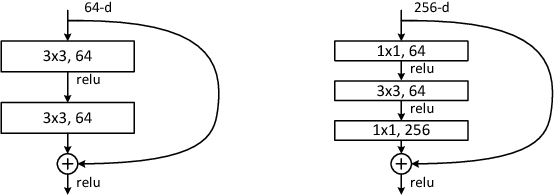
\includegraphics[width=.667\textwidth]{images/Chapter2/6-Figure5-1.png}
\caption{A residual block with two convolutions (\textit{left}) and three convolutions (\textit{right}). After the convolutions, the identity of the layer's input is added before an activation function and the next layer \citep{He_2016}.} 
\label{fig:resid}
\end{figure}

The main idea is to provide the deeper layers with information gathered before in order to not get lost in parameters the deeper the signal goes into the network. This is achieved by the identity function. After a convolutional layer, the identity from the last activation is added to the new activation,  allowing a massive improvement in network depth. The authors provide 34-(\autoref{fig:Res34}), 50-, 101- and 152-layer networks. The 34-layer network used the residual structure from \autoref{fig:resid} (\textit{left}) while the other architectures are based on the structure from \autoref{fig:resid} (\textit{right}). It's also worth noting that ResNet is not using dense nets at the end of the convolutional layers apart from the 1000 class dense net to receive probabilities for the image classification. It was shown that these fully connected layers were not needed for high accuracies and only increased the number of parameters unnecessarily. While the best VGG achieved a $6.8\%$ top-5 error rate in the 2015 ILSVRC, ResNet-34 already was beating this with a $5.6\%$ top-5 error. The deeper the network, the lower the error was and ResNet-152 was able to score an outstanding $3.57\%$ error, beating even human image classification with approximately $5.1\%$ top-5 error accuracy \citep{russakovsky2015imagenet}.

